We extended the visulaizer to fully comply with Raft protocol
implementing missing functionalities, like cluster memberships changes.
We also improved the interface (Figure~\ref{fig:final}) and cleaned up the codebase.

\subsection{Simulation model}
Fixing the problem in Section~\ref{sec:simulation} is not straight forward: swapping the two checks would
break other scenarios (\texttt{e.g.} a leader message is due just after the \texttt{ElectionTimeout}).
The only definitive fix would have been rewriting the entire simulation system.
Given the use case and applications of Raft Scope we decided to limit the maximum speed to prevent such problems.

Network noise was integrated into the simulation and the state object, dropping each message with a probability
set by the user.

\subsection{Interaction}
\emph{Cluster membership changes} are an important part of a consensus protocol.
Raft initially handled this with a procedure called \emph{joint consensus}
but Ongaro expanded on this matter, in the Chapter 4 of his Ph.D. thesis~\cite{ongaro2014consensus},
with a new simpler algorithm that only allows single server changes at a time (both removal and addition).
However any arbitrary change that could be expressed with joint consensus
can be also managed with a series of single server changes that is easier to visualize.
Each configuration in the series must be committed before the next one can take place.
With the intention to clarify this series of changes, we added a \emph{cluster configuration changes queue}.
This queue keeps track of all the cluster reconfigurations submitted by the user while they are being processed.
The original dissertation is not clear on what action to take regarding pending configurations when leadership is lost.

A bug in the single server membership change algorithm was later found and discussed in the raft-dev mailing list~\cite{bug} which
could rewrite committed history. The bug occurred whenever leadership was lost and two pending configurations were happening
at the same time, submitted by different leaders. As described there, we implemented the fix by having leaders append a \texttt{NOOP} to their log.

We implemented a safety check for disruptive (removed) servers as described
in Section~4.2.3 of the author's thesis.
Servers, when removed, could disrupt cluster functionality by starting new
elections whenever a pending change for their removal
is being processed. The fix makes servers ignore VoteRequest RPCs if they have received an heartbeat within
\texttt{MIN\_ELECTION\_TIMEOUT} from an active leader.

\subsection{Integrating the new features}
In order to allow transparent playback we modified the rendering phase in the main loop to take in account the possibility for
membership changes and automatic message drop due to network noise.
It was particularly challenging to determine when it is safe to remove a server
from the simulation: it is not correct to remove it when its corresponding configuration change is committed because
other servers, which have not yet received the entry, might still interact with it.
We decided to remove it when every other server has removed it from its \texttt{peers} list.

\subsection{Code reorganization}
We added two more scripts: \texttt{render.js} and \texttt{presenter.js}.

The first handles all the graphic related tasks, in particular SVG generation,
servers realignment, sliders and log table updates.
It also contains the code that generates modal and context menu when
the user clicks on a message or a server.

The \texttt{presenter.js} file contains utilities to save and load simulation scenarios (state).
Further it provide hot keys to quickly interact with the system, offering the
functions that help simulate interesting situations such as split votes.\\

Thanks to our refactoring the \texttt{script.js} now only contains the
initialization code and the \emph{system clock} loop.


\subsection{Interface}
The log table has been rewritten in plain \texttt{html} instead of SVG
to allow support for an infinite log with auto scrolling and a high number of servers.
To avoid confusion the ``leader only'' fields in the modal menu of the
follower servers have been hidden and a legend was added to explain the
otherwise cryptic symbols in the log table. Moreover, each log entry
is categorized depending on its type (\texttt{NOOP}, configuration change entry, user request).

We added controls for the features we introduced in the protocol: a slider to set the \emph{network noise}, a \emph{server add} button, a button to the server context menu for removal and finally a new table to visualize the cluster configuration changes queue.

\begin{figure}[h!]
    \centering
    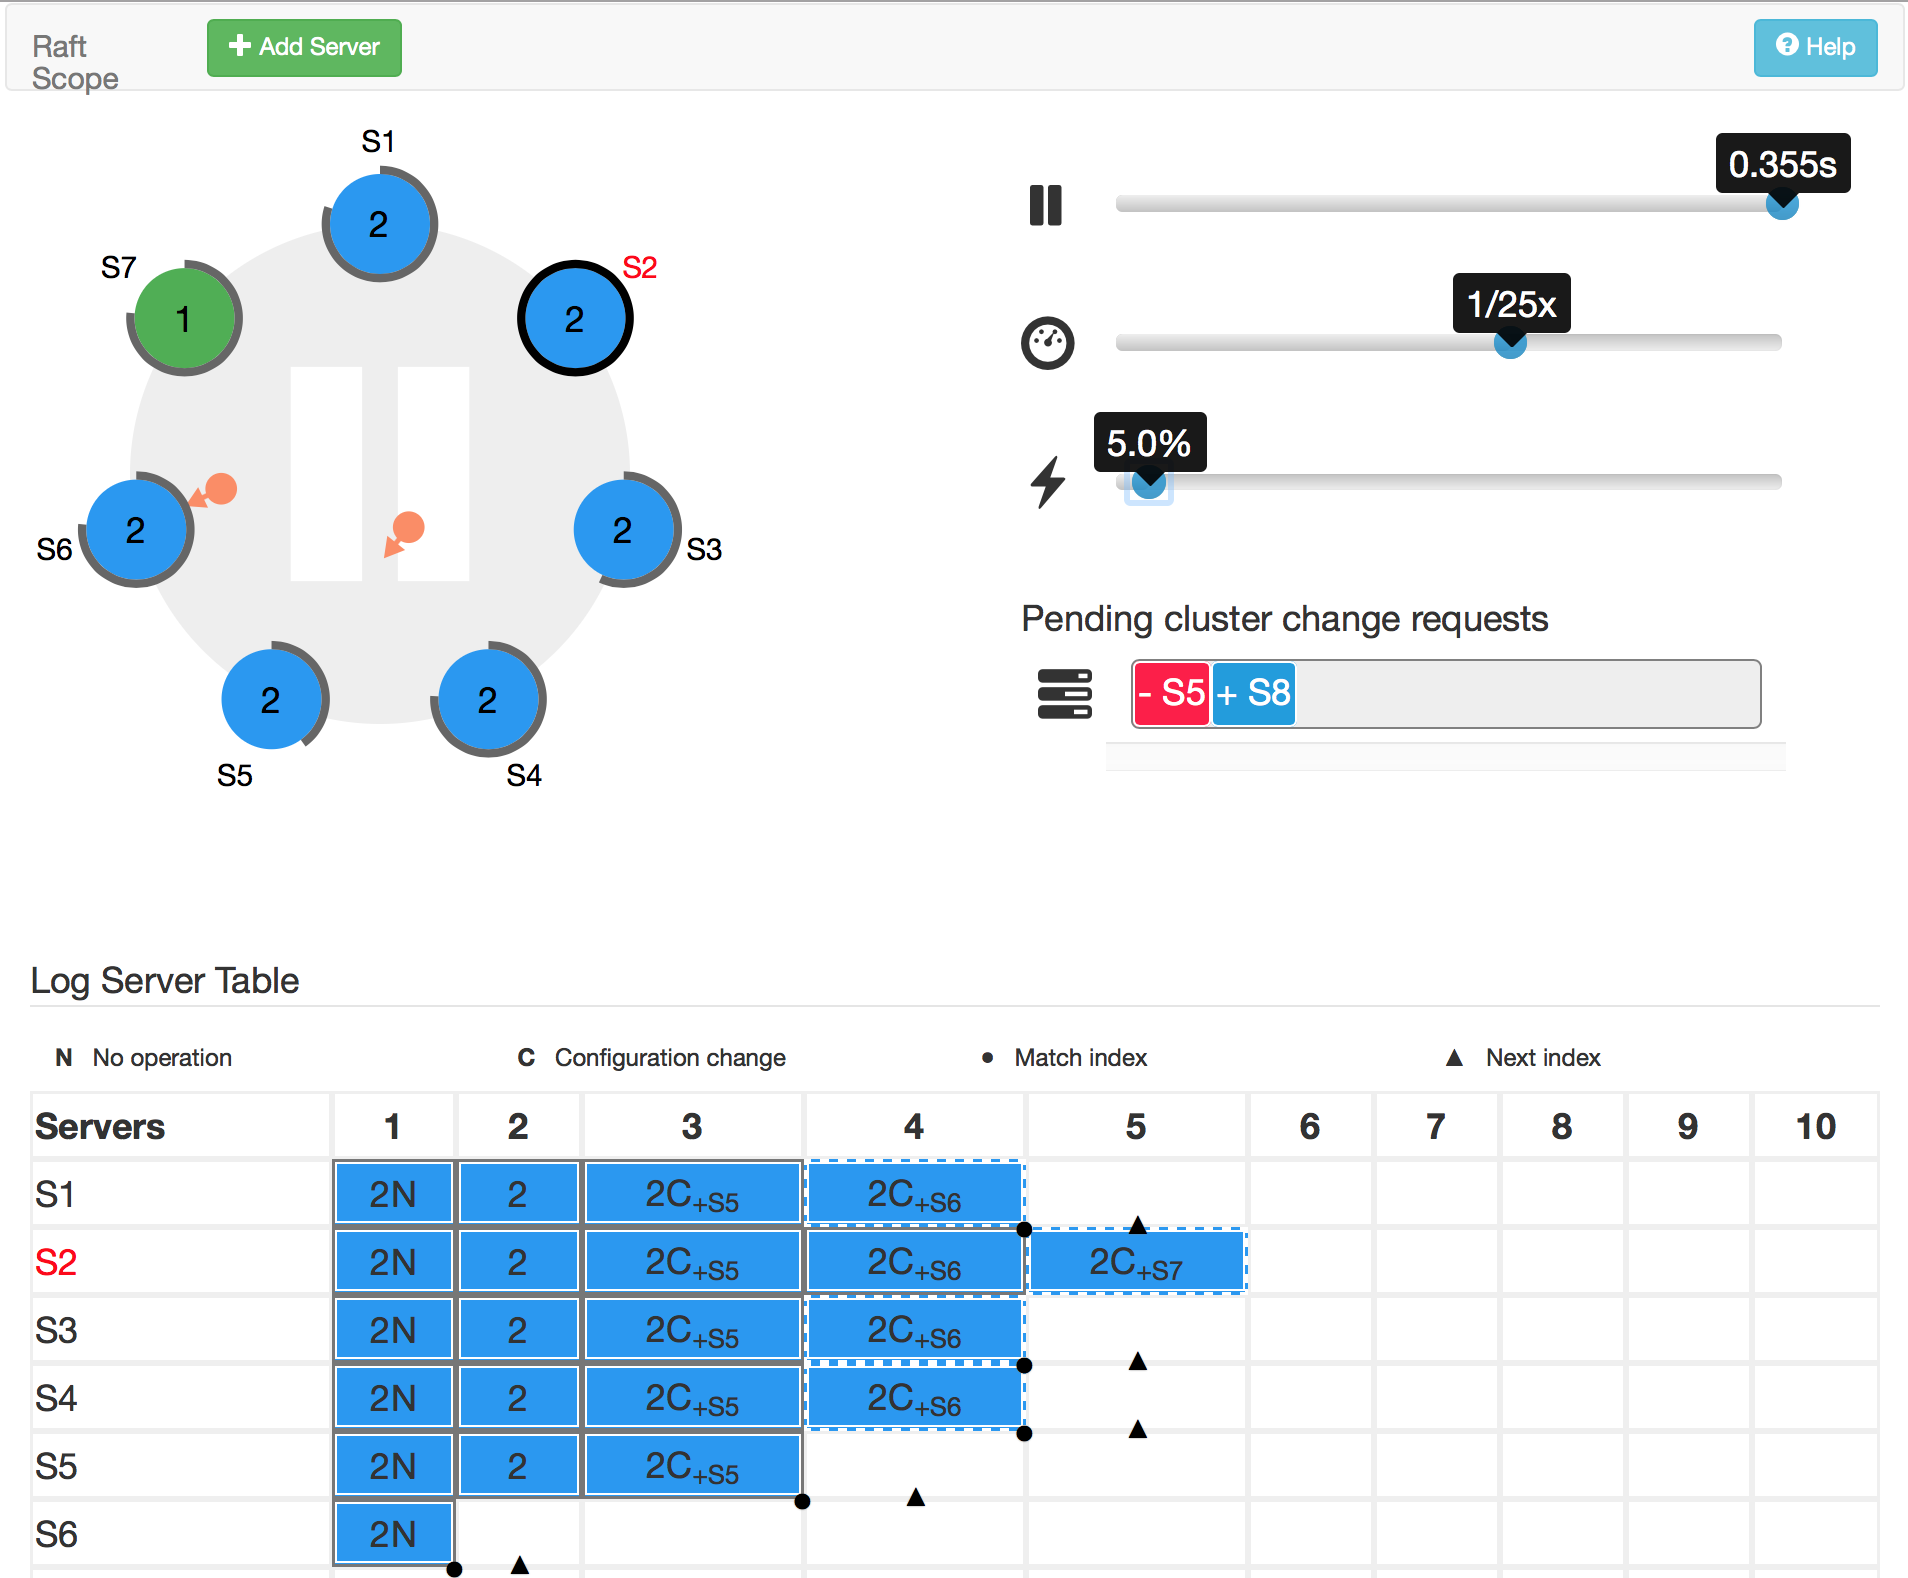
\includegraphics[width=0.9\linewidth]{our.png}
    \caption{Extended}\label{fig:final}
\end{figure}
